
\documentclass[12pt]{nuthesis}	% The nuthesis class is based on 
				% amsbook.cls.

\usepackage{graphicx}
\usepackage{algpseudocode}
\usepackage{algorithm}
\usepackage{amsmath}
\usepackage{amssymb}
%\usepackage{subfigure}
\newcommand{\argmin}{\operatornamewithlimits{arg\ min}}
\usepackage{xcolor}
\usepackage{multirow}
\usepackage{multicol}
\usepackage{makecell}
\usepackage{caption}
\usepackage{subcaption}
\usepackage{soul}

\newtheorem{prop}{Proposition}

% DATA OF AUTHOR AND DISSERTATION %


\author{Aleksandra Kalinowska}

\title{Shared Control for Robot-Aided Task Training and Robotic Assistance}

\degree{MASTER OF SCIENCE}  % Default: DOCTOR OF PHILOSOPHY
\field{Mechanical Engineering}
\graduationmonth{December} 
\graduationyear{2018}  

\begin{document}

\frontmatter		% Preliminary pages start here.
\maketitle		% Produces the title page.
\copyrightpage		% Creates the copyright page.

\abstract		% Abstract.
Robots have the potential to assist with both learning and executing difficult tasks, particularly in populations with motor deficit. However, adequate shared control schemes are needed to effectively allocate control between the human and the user to either facilitate training or provide assistance without unnecessarily limiting the user's intended actions. Here, we propose a shared control paradigm based on filtering that can be used for both training and assistance in human-robot interfaces with known tasks. We use a novel criterion for evaluating user input---the mode insertion gradient (MIG), commonly used in hybrid control---that allows us to instantaneously assess the impact of user actions on the evolution of a dynamic system over a time window into the future. As a result, the filter is permissive to many chosen strategies and minimally interfering---qualities desired when evaluating human actions.

We explore a version of the shared control paradigm for assistance. We show in simulation that it is able to assist in task completion and enforce safety even for unskilled users simulated with Gaussian noise input. At the same time we show that, when possible, the interface remains transparent to users, particulary skilled users simulated using near-optimal model predictive controllers. Finally, given a stable controller for providing assistance, we show that this filter-based shared control scheme can to first order guarantee system safety with respect to a pre-defined objective. Future work will involve implementing the shared control paradigm for real-time assistance on hardware devices, such as a lower-limb exoskeleton.

In parallel, we explore the shared control paradigm for task training. Through a human subject study, we show significant improvement in task learning using the proposed scheme. For the task of inverting a simulated cart pendulum, users continually improve when training with this filter-based feedback, while controls plateau shortly into the training and overall reach a lower skill level. Interestingly, we observe the shared control paradigm to exhibit multiple features that have, in previous studies, been shown to be conducive to learning. For one, it only rejects user actions, allowing failure at the task and avoiding user passivity. Secondly, it improves performance when actively engaged. And thirdly, it is sensitive to user skill level and real-time performance, behaving similarily to traditional assist-as-needed paradigms. Further experiments will involve studies of impaired individuals in clinically relevant tasks as well as direct comparisons with other assist-as-needed shared control schemes. 

Overall there is significant interest in enabling difficult tasks or making them safer through online robotic assistance as well as in facilitating task training through forceful robotic interaction---the proposed filter-based shared control paradigm with MIG as an evaluation criterion can facilitate these human-robot collaborations. 


\acknowledgements	% Acknowledgements (optional).

acknowledgements here

% \preface		% Preface (optional).

% This is the preface.


%% A few more optional pages (uncomment if needed)
%
%\listofabbreviations 
%
%This is the list of abbreviations (optional).
%
%\glossary
%
%This is the glossary (optional).
%
%\nomenclature
%
%This is the nomenclature (optional).
%
%% Note that the dedication text must be passed as an argument
%% of the \dedication command
%\dedication{This is the dedication (optional).}
%

\clearpage\phantomsection % needed for the hyperlinks to work correctly
\tableofcontents	% Table of Contents will be automatically
			% generated and placed here.

\clearpage\phantomsection % needed for the hyperlinks to work correctly
\listoftables		% List of Tables and List of Figures will be placed

\clearpage\phantomsection % needed for the hyperlinks to work correctly
\listoffigures		% here, if applicable (optional).



\mainmatter             % Actual text starts here.

%%%%%%%%%%%%%%%%%%%%%%%%%%%
% Actual text starts here %
%%%%%%%%%%%%%%%%%%%%%%%%%%%

% If there is an introduction it must be the first chapter

\chapter{Introduction}	% The first chapter.
\label{chapter: intro}


Shared control algorithms have been developed for robotic assistance and robot-supported training in applications ranging from assisted vehicle navigation~\cite{autovehicle2014} and surgical robotics~\cite{surgeryrobot2004,RSS_surgery2014} to brain-computer interface manipulation~\cite{teleBCI2017} and exoskeleton-assisted gait~\cite{RSS_exo2013, exoMPC2011}. The aims and safety requirements of these systems vary greatly, but one challenge is often the same---how do we most effectively allocate control between the user and the machine? 

User trust in the robot is a critical factor in the overall performance of the joint human-machine system \cite{measurement_of_trust}. Trust, in this context, mainly depends on robot performance and its attributes, such as dependability, predictability, and level of automation \cite{trust_factors}. Thus, to encourage user trust, shared control algorithms should avoid robot behavior that is difficult for the human to understand~\cite{RSS_RoboObj2017}, unpredictable, or unnecessary. In task-based assistance, avoiding such behavior can be challenging, because there are often many ways of accomplishing a task and the individual is likely to take an approach that is different from the controller’s calculated strategy. However, the issue can be addressed by developing shared control paradigms that instantenously adjust to operator performance and real-time adapt to varying user strategies, such as in~\cite{RSS_shah_adaptive} and in the work proposed here.

Another factor to consider is user preference. In~\cite{RSS_userpref2017}, machine learning techniques were used to model user preferences for autonomous systems; in other approaches, users were able to manually choose their level of assistance~\cite{exoskeletons}. In general, studies show that users of assistive devices prefer to maintain as much control authority as possible~\cite{argall_keynote,RSS2011_assistedteleoperation,lankenau2001}. Overconstraining user inputs may prevent them from utilizing valid control strategies and hence leads to frustration and device abandonment~\cite{survey_deviceabandonment}. That said, users may be willing to accept some loss of control authority, but only if the improvements in performance are significant~\cite{RSS2011_assistedteleoperation, lankenau2001}. Therefore, devices are most likely to be used if they make tasks significantly easier without limiting users' actions~\cite{survey_deviceabandonment}. 

% For instance, strict obstacle avoidance controls prevent wheelchair users from making maneuvers that bring them too close to a wall~\cite{lankenau2001}.

Finally, in robotic training, providing too much assistance or overconstraining users undermines the therapeutic impact of the device. Engaging the user has been shown to be critical to robotic training~\cite{marchal2009}. Likewise, allowing mistakes or errors and overall task failure has been shown to be critical to learning~\cite{thoroughman2000learning}. In some cases, successful interfaces have adopted strategies of amplifying error~\cite{emken2007motor, patton2006evaluation}. On the flip side, interfaces that provide too much support oftentimes lead to user passivity, resulting in low skill retention and little transferable skills~\cite{schmidt1992new, winstein1994effects}. 

Many shared control schemes adapt their level of support online~\cite{emken2008,riener2005,wolbrecht2008, ellis2009} using an algorithm or schedule that prescribes changes based on some notion of the user's need for assistance. These levels of support can be modulated based on performance measures such as error~\cite{fisher2014,marchal2009, reinkensmeyer2016intro,patton2006error}, movement speed~\cite{kahn2004}, and task adeptness~\cite{krebs2003}, or based on the user's strength and fitness level~\cite{lokomat_clinical_study,RSS_exo2013} or current cognitive engagement in the task \cite{assistance_in_distraction}. At other times, the level of support can be manually adjusted by a physical therapist or the users themselves \cite{exoskeletons}. These adaptive shared control schemes are often referred to as assist-as-needed and are characterized by dynamically updating the relative contributions of the robot and human.

Here, we present a filter-based assist-as-needed shared control paradigm. While other assist-as-needed schemes adjust the level of provided support from trial-to-trial, we implement a filter that acts based on real-time assessment of user intent. It requires no predefined trajectory, runs on an indefinite time horizon, and automatically adapts to operator skill. \textit{A key contribution of this work is the criterion used for evaluating and selecting admissible user input.} As our criterion, we use the Mode Insertion Gradient (MIG)---a concept from hybrid control that allows us to assess how users' inputs affect the human-machine system over a time window into the future. 

The result is a mechanical filter that remains transparent when users are skilled and high performing, allowing inputs that are safe and/or do not hinder achieving a task goal, but interferes when users are underperforming, disallowing inputs that are unsafe or incorrect with respect to the task objective. It is worth noting that the filter requires user input and does not drive the system when the user is not actively engaged in the task, encouraging user engagement. It also does not require pre-defining a desired trajectory, allowing subjects to explore various strategies for completing a task. 

In chapters to follow, we present experimental results on the performance and training effects of this real-time assist-as-needed shared control scheme. We evaluate the MIG-based filter in two modes: assistance and training. In the assistance mode, we replace ``incorrect" user inputs with a controller-calculated action to impose safety and/or task completion. In the training mode, we reject ``incorrect" user actions to allow failure and facilitate learning. Experimental and theoretical analyses of the shared control scheme in both modes are presented in Chapters~\ref{chapter: assistance}~and~\ref{chapter: training}, respectively. We demonstrate the assist-as-needed feature of the filter by evaluating correlations between initial user skill level and current user performance on the one side and controller engagement on the other. We conclude our work and suggest future steps with a discussion in Chapter~\ref{chapter: conclusions}. A large part of the results was published in June 2018 in the Proceedings of Robotics: Science and Systems \cite{myRSS_MIGMDA}. 

%Through a healthy human subject study, we show a correlation between user skill-level and the acceptance rate of the algorithm. Because we do not simply compare the user and controller decision at each time instance, we avoid the pitfall of arbitrarily rejecting actions that do not align with the controller's strategy but otherwise bring the system closer to a target configuration. In a sense, trust in the user is implicitly represented in the algorithm through the instantaneous assessment of user actions. Therefore, there is no need to implement an adaptive scheme that explicitly assesses user trustworthiness over time. Finally, in the human subject study ($n=28$), we observe that a MIG-based filter exhibits a training effect compared to training with no assistance for the tested group; in simulation, we demonstrate that a filtering algorithm utilizing a MIG criterion succeeds in task completion even with Gaussian noise inputs for two dynamic tasks---cart-pendulum inversion and SLIP balancing, while intervening minimally and remaining flexible with respect to the user's approach strategy. 


%\chapter{Related Work}
%\label{chapter: relatedwork}
%\input{chap2_relatedwork.tex}

\chapter{Background and Methods}
\label{chapter: methods}	


\section{Filter-Based Shared Control}

\subsection{Maxwell Demon's Algorithm}

The Maxwell's Demon Algorithm (MDA) is a combined filter-controller computational unit that operates similar to the philosophical Maxwell's Demon from thermodynamics in that it accepts selected actions that meet a pre-defined criterion and disallows others. Specifically, it allows control actions that drive a system towards a pre-specified desired objective and disallows actions that drive the system away from that objective. The algorithm was originally proposed in \cite{MDA_Emmanouil} by Tzorakoleftherakis and Murphey, where the authors demonstrate that even noisy inputs, generated using i.e. a Gaussian distribution, can be a rich source of control authority if filtered in a meaningful manner. 

The algorithm was further developed by Fitzsimons et al. \cite{MDA_Katie} as a shared control paradigm for joint human-robot systems. In that work, authors show that MDA is able to improve task performance for technology-assisted tasks by simply rejecting ``wrong" user inputs (rather than actively assisting in task completion). In the study, 9 subjects attempt the task of inverting a simulated cart-pendulum with MDA-based feedback. They achieve better performance at the task when controlling the system with either an MDA-based software filter or MDA-based haptic feedback, providing initial results that MDA could be applied to design useful human-machine interfaces. 

In this work, we build on the idea of using MDA for shared control. We discriminate and evaluate two application scenarios and hence define two respective MDA modes: training and assistance. In training mode, if user actions are rejected, no control is applied to the system; in assistance mode, if user inputs are rejected, they are replaced with a controller-calculated action---this principle is illustrated in Fig.~\ref{fig: accept_reject_replace} on the example of a hand pushing a mass. 

In training mode, MDA improves task performance but allows for failure at the task without a rich enough input, making it well suited for robot-aided task training, where active engagement and failure are conducive to learning. Assistance mode, on the other hand, shows promise for being useful in allocating control of assistive devices, where safety and/or task success are of utmost importance. As mentioned above, we evaluate MDA in both modes---in training mode in Chapter~\ref{chapter: training}, and in assistance mode in Chapter~\ref{chapter: assistance}. 

\begin{figure}[h]
\centering
\includegraphics[width=0.7\columnwidth]{MDAconcept.pdf}
\caption{Filter-based robotic responses on the example of a hand pushing a mass. The robot filters user input by physically accepting, rejecting, or replacing it. When a user action is accepted, the robot admits the force. When a user action is not accepted, the robot either rejects it by applying an equal and opposite force or replaces it by applying a force, such that the net effect on the system is equal to the controller-calculated input. }
\label{fig: accept_reject_replace}
\end{figure}



\subsection{Mode Insertion Gradient (MIG) as a Criterion}
\label{criterion}

In shared control applications, a key part of the Maxwell's Demon Algorithm is the criterion used for evaluating user actions. In both \cite{MDA_Emmanouil} and \cite{MDA_Katie}, MDA was implemented with a criterion based on a direct comparison of user actions to the actions calculated by an optimal controller. In the studies presented here, we instead use the Mode Insertion Gradient (MIG) as an evaluation criterion of user inputs, which allows us to give users more flexibility in the way they approach a task. 

Usually, the MIG $ \frac{dJ}{d\lambda}$ is used, in mode scheduling problems, to determine the optimal time $\tau$ to insert control modes from a predetermined set ~\cite{egerstedt2006,modesched2012,vaseduvan_switchsys2010, alex_SAC, caldwell2016}. Here we use the mode insertion gradient,
\begin{equation}\label{mig}
    \frac{dJ}{d\lambda}(\tau)=\rho(\tau)^T \left[f(x(\tau),u_2(\tau))-f(x(\tau),u_1(\tau))\right],
\end{equation}
as a measure of the sensitivity of the cost to a change from the nominal control, $u_1$, to a particular user input, $u_2$. In (\ref{mig}), state $x$ is calculated using nominal control, $u_1$, and $\rho$ is the adjoint variable calculated from the nominal trajectory $x(t)$,
\begin{equation*}
    \dot \rho = -\nabla l_1(x)-D_xf(x,u_1)^T\rho,
\end{equation*}
where $l_1(x,t)$ is the incremental cost and $\rho(t_f)=\nabla m(x(t_f))$. Moreover, in the work presented here, we define the nominal control, $u_1$, to be equivalent to a null action ($u_1(t) = 0$), and we define $u_2$ with the piece-wise function below,
\[ u_2(t) =  \left\{
		\begin{array}{ll}
  			u_{user} & t\leq t_s \\
  			u_1 & t_s\leq t\leq T \\
		\end{array} 
\right. \]
where $t_s$ is the sampling time, $T$ is the time window over which we are evaluating system behavior, and $u_{user}$ is a user input recorded at current time $t$. It is worth noting that, in future work, $u_2$ could instead be defined by a combination of user input at current time $t$ and actions from an optimal controller over time $T$ into the future. This would add further flexibility to the criterion and give the user more control authority over the joint system, because any user action that could be corrected for by a future optimal action or sequence of optimal actions without destabilizing the system during the time window $T$ would be admitted.  

When using MIG as an evaluation criterion, we calculate the integral of the mode insertion gradient over a time window $T$ into the future
\begin{equation}\label{mig_int}
    \int_{t_{now}}^{t_{now}+T}\frac{dJ}{d\lambda}(t)\delta t,
\end{equation}
to evaluate the impact of user control $u_2$ on the system over time $T$. We show that, when negative, the integral indicates that $u_2$ is a descent direction over the entire time horizon, and thus can serve as the basis for evaluating the impact of a current user action on the evolution of a dynamic system over that time window into the future. Moreover, stability can be inferred if (\ref{mig_int}) satisfies a contractive constraint \cite{contractive, iSAC}. 

\noindent\begin{minipage}{\columnwidth}
\renewcommand\footnoterule{} 
\begin{algorithm}[H]
	\caption{A filter with MIG criterion.}\label{algo}
	\noindent\footnotetext{\noindent\normalsize *Note that the filter can be used with any model predictive controller (MPC) that can complete the task. Here a controller similar to the conjugate gradient descent method\cite{conjugate_gradient} was used.}
		    \\         
        Set sampling time $t_s$ and time horizon $T$. Set mode $m$ to either training $(T)$ or assistance $(A)$. Define objective function for filter and controller.
		\begin{algorithmic}[1]
			\While {$t_0 \leq t_f$}
			\State Infer user control vector $u_{user}$ from sensor data
			\State Simulate $x(t)$ and $\rho(t)$ in $[t_{now}, t_{now} + T]$ assuming \[ u =  \left\{
			\begin{array}{ll}
      			u_{user} & t\leq t_s \\
      			0 & t_s\leq t\leq T \\
			\end{array} 
			\right. \]
			\State Compute $\int \frac{dJ}{d\lambda}$
			\If {$ \int \frac{dJ}{d\lambda} \leq 0$}
			\State $u_{now} = u_{user}$
			\Else
			\If {$m=T$}
			\State Assign controller value
			$ u_{now} = 0 $
			\ElsIf {$m=A$}
			\State Calculate optimal control $u_{controller}$*
			\State Assign controller value 
			$ u_{now} = u_{controller} $
			\EndIf
			\EndIf
			\State Apply $u_{now}$ for $ t \in [t_{now}, t_{now}+t_s]$
			\EndWhile
		\end{algorithmic}	
	\end{algorithm}
	\renewcommand\footnoterule{}
\end{minipage}
\vspace{0.7cm}

In our experimental study, we utilize the MIG criterion in a filter-based shared control scheme. For an outline of the approach, refer to Algorithm \ref{algo}. 


\section{Simulated Users}
\label{section: simulated users}

%\begin{figure}[h]
%\begin{subfigure}{0.45\textwidth}
%\centering \captionsetup{width=0.9\linewidth}
%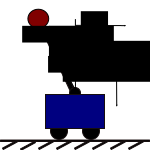
\includegraphics[width=\linewidth]{cart-pend.pdf}
%\caption{Subject Specific Trends}
%\end{subfigure}
%\begin{subfigure}{0.45\textwidth}
%\centering \captionsetup{width=0.9\linewidth}
%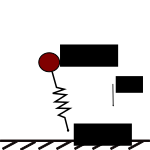
\includegraphics[width=\linewidth]{SLIP.pdf}
%\caption{Mean Across Subjects}
%\end{subfigure}
%\caption{\textbf{Percent of Accepted Actions} There are no discernible trends in Controller Engagement over time.}
%\end{figure}

\begin{figure}[h]
\centering \captionsetup{width=0.45\linewidth}
\begin{multicols}{2}
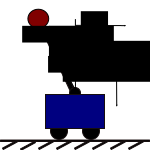
\includegraphics[width=0.9\columnwidth]{cart-pend.pdf}
\caption{The cart-pendulum system with state vector $x=[\theta, \dot{\theta}, x_c, \dot{x_c}]$ and horizontal acceleration of the cart as control input.}
\label{fig: cartpend-schematic}
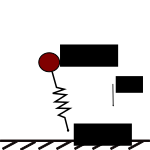
\includegraphics[width=0.9\columnwidth, keepaspectratio]{SLIP.pdf}
\caption{The SLIP model with state vector $x = [x_m, \dot{x}_m, z_m, \dot{z}_m, x_t]$ and control vector $u = [u_s,u_t]$, where $u_s$ is the leg thrust applied during stance and $u_t$ is the toe velocity control applied during flight.}
\label{fig: slip-schematic}
\end{multicols}
\end{figure}

To test the proposed algorithm in assistance mode, we run experiments with simulated users. We use Gaussian noise as well as a Model Predictive Controller (MPC) with differing objective functions to simulate users of varying skill levels. Specifically, an objective function defined as 
\begin{equation}
J = \frac{1}{2} \int_{t_o}^{t_f} \lVert x(t) - x_d(t)\rVert_{Q}^2 + \lVert u(t) \rVert_{R}^2 \delta t,
\end{equation}
with $Q \ge 0$ and $R \ge 0$ being metrics on state error and control effort and $x_d(t)$ being the desired trajectory is used in the simulated experiments. The systems and specific objective functions are described in the sections below. 


\subsection{Cart-Pendulum Task}

A cart-pendulum system as illustrated in Fig.~\ref{fig: cartpend-schematic} is one of the systems used. It has a state vector $x=[\theta, \dot{\theta}, x_c, \dot{x_c}]$ and a horizontal acceleration of the cart $u$ as control input. The task associated with this system is to invert the pendulum to its unstable equilibrium, where $\theta = 0$ and $\dot{\theta} = 0$. 

\begin{figure}[h]
	\begin{center}
		\includegraphics[width=0.6\columnwidth, keepaspectratio]{cp_table.pdf}\par
	\end{center}
\caption*{}
\vspace{-1.3cm}
\label{table_cp}
\end{figure}

To create the simulated skilled users, we utilize an MPC with objectives representing successful inversion strategies. An example objective includes inverting the cart-pendulum while minimizing energy and staying close to the origin---the exact function parameters are given in Table 1. To approximate an unskilled user, we generate noise input, using a Gaussian distribution within the saturation limits. While we made the above choices, there are other reasonable alternatives for representing simulated users.

In either case, we then filter user actions using a MIG-based algorithm with a high-level objective function also listed in Table 1. For the MIG filter, we choose to place a high weight only on the angle $\theta$. The goal is to emphasize the task of inversion while minimally limiting users' varying approach strategies.


\subsection{SLIP Hopper}

Another system used is the spring-loaded inverted pendulum. The SLIP is a hybrid, low-dimensional system that has been shown to be a reliable approximation of human running \cite{SLIP_for_running_nature} and is therefore used to model running dynamics in robotic locomotion \cite{SLIP_robot_evidence}. Here, a 2D SLIP model (Fig.~\ref{fig: slip-schematic}) is tested with a state vector described by $x = [x_m, \dot{x}_m, z_m, \dot{z}_m, x_t]$, where $x_m$ and $z_m$ are the coordinates of the mass, and $x_t$ is the coordinate of the toe, and a control vector described by $u = [u_s,u_t]$, where $u_s$ is the leg thrust applied during stance and $u_t$ is the toe velocity control applied during flight. Hybrid dynamics of the form
\begin{align*}
    f_{stance}= 
    \begin{pmatrix}
    \dot{x}_m \\
    \frac{(k(l_0-l_s)+u_s)(x_m-x_t)}{ml_s} \\
    \dot{z}_m \\
    \frac{(k(l_0-l_s)+u_s)z_m}{ml_s} - g \\
    0
    \end{pmatrix}
\end{align*}
and $f_{flight} = (\dot{x}_m,0,\dot{z}_m,-g,\dot{x}_m+u_t) $
are used. Parameters $k$, $l_0$, and $m$ describe the SLIP model spring constant, resting spring length, and mass, respectively. All parameters were given a value of 1 in our simulations. 

To determine switches between stance and flight modes, a guard equation $\phi(x)$ is employed
\begin{equation*}
    \phi_{stance \rightarrow flight}(x) = \phi_{flight \rightarrow stance}(x) = x_m - \frac{l_0}{l_s}z_m
\end{equation*}
with $l_s$ being the leg length during stance
\begin{equation*}
    l_s=\sqrt{(x_m-x_t)^2+z_m^2}.
\end{equation*}

In the experiments, we again use input from simulated users of different skill level, which we generate using MPC with objective functions outlined in Table 2. We approximate an unskilled user using Gaussian noise; a low-skill user using MPC with a height objective lower than the spring length, which causes the SLIP to fall if simulated without assistance; and a skilled user using MPC with a feasible objective such that the controller can achieve forward motion without assistance. 

\begin{figure}[h]
	\begin{center}
		\includegraphics[width=0.6\columnwidth, keepaspectratio]{SLIP_table2.pdf}\par
	\end{center}
\label{table_slip}
\end{figure}

Here, the MIG-based filter uses a high-level objective function defining the height of the center of mass $z_m$, also listed in Table 2. The goal is to emphasize the safe upright orientation of the SLIP hopper while minimally limiting its movements and velocity in the $x$-direction.


\section{Human Subject Experiments}
\label{section: human experiments}

In addition to testing simulated users, we conducted a human subject study, where we implemented and tested the proposed shared control paradigm in the form of a mechanical filter. Subjects used an upper limb robotic platform as an interface to control a simulated cart-pendulum system. During experimental trials, users were instructed to invert the pendulum to its unstable equilibrium and keep it there for as long as possible. User input was inferred from a force sensor at the robot's end-effector and was continually evaluated at 100Hz. During trials when the filter was engaged, user actions were either accepted or rejected based on the criterion described in Section ~\ref{criterion}. 


\subsection{Experimental Platform}

All human subject data was collected using the robotic platform shown in Fig.~\ref{nact3d}. The device is a powerful haptic admittance-controlled robot that can be used to render virtual objects, forces, or perturbations in three degrees of freedom. It is similar to the robotic platform used in \cite{ellis2016} and \cite{stienen2011} to provide a means to modulate limb weight support during reaching and to quantify upper limb motor impairments in stroke survivors.

\begin{figure}[h]
\centering
\includegraphics[width=0.7\columnwidth]{NACT-userview-small.png}
\caption{(top) Upper limb robotic platform used during experiments. (bottom) The platform provides haptic feedback to simulate a specified inertial model via an admittance control scheme. A voluntary force $f(s)$ is measured by a force-torque sensor at the end-effector and passed through a model $M(s)$ that determines velocity $v_r(s)$ at which the robot should move. The reference velocity is tracked by the low level velocity controls, $C(s)$, of each motor drive. In addition to a force input, the user delivers involuntary impedance forces due to movement, given by dynamics $H(s)$. Acceleration information is fed back as a pseudo-force $sm_a$ for extra inertia reduction of the system.}
\label{nact3d}
\end{figure}

During the experiment, each subject was seated in a Biodex chair with their arm secured in a forearm-wrist-hand orthosis. The orthosis could rotate passively, and the device could move its end-effector within a workspace defined both by its design limits and limits set by the investigators. At the point where the orthosis was mounted, a force-torque sensor measured subject input, which was then fed back to the admittance controller. In our experiments, the device was set up to physically support the upper limb of the participant in the z-direction while allowing them to move freely on the x-y plane. 

During testing, a display provided real-time visual state feedback to the user about the cart-pendulum system they were attempting to invert. High stiffness virtual springs in the haptic model were used to restrict user motion to a horizontal plane corresponding to the path of the cart in the virtual display. When user inputs were accepted, the control scheme behaved as described in Fig.~\ref{nact3d} and the end-effector motion changed according to the applied force. When user inputs were rejected, the measured user input $f(s)$ was ignored in the control scheme, such that the robot continued to move under its predefined dynamics as if no force had been applied by the user.

\subsection{Experimental Protocol} 

Twenty-eight subjects (9 males and 19 females) consented to participate in this study.\footnote{This study protocol was approved by the Institutional Review Board and all participants signed an informed consent form.} All subjects completed three sets of thirty 30-second trials with short breaks between sets. Each trial consisted of the subject attempting to invert a simulated cart-pendulum system, using cart acceleration as input. At the beginning of each session, the system and task was demonstrated to the subject using a video of a sample task completion. Subjects were instructed to attempt to swing up the simulated pendulum to the upward unstable equilibrium and balance it there for as long as possible. Subjects were instructed to continue to try to do this until the 30 seconds were over even if they succeeded at balancing near the equilibrium at some point throughout the trial.

Upon enrollment, subjects were randomly placed into either a control ($n=10$) or training group ($n=18$). During the second set, feedback in the form of a filter was engaged for the training group, while the control group completed each of the three sets without any feedback. Again, each user did three sets of thirty trials: set 1 (both groups: no feedback), set 2 (control: no feedback, training: feedback in the form of a mechanical filter), set 3 (both groups: no feedback). The experimental protocol is illustrated in Fig.~\ref{fig: exp_protocol}.

\begin{figure}[t]
\centering
\includegraphics[width=0.7\columnwidth]{Exp_Protocol_MIG.pdf}
\caption{Experimental Protocol. Upon enrollment, subjects were randomly placed into either a control ($n=10$) or training group ($n=18$). Each session consisted of three sets of thirty trials (each block above represents one such set). In set 1, both groups received no feedback, in set 2 the control group trained without feedback while the training group trained with feedback in the form of a mechanical filter, and in set 3 both groups attempted the task again with no feedback.}
\label{fig: exp_protocol}
\end{figure}



\subsection{Performance Measures}\label{metrics}

Several measures were calculated to quantify user performance in individual trials. Specifically, time to success, balance time, and error were calculated for all trials and subsequently each trial was classified as successful or unsuccessful. 

A trial was considered successful when a subject reached an angle of $\pm0.4$~rad and angular velocity of $\pm0.75$~rad/s for at least 2 seconds. This success definition was used to determine the success rate and time to success of the users in each set. In addition, if a subject was successful, the total time spent at an angle of $\pm0.4$~rad and angular velocity of $\pm0.75$~rad/s 
\begin{figure}[!h]
\begin{center}
  	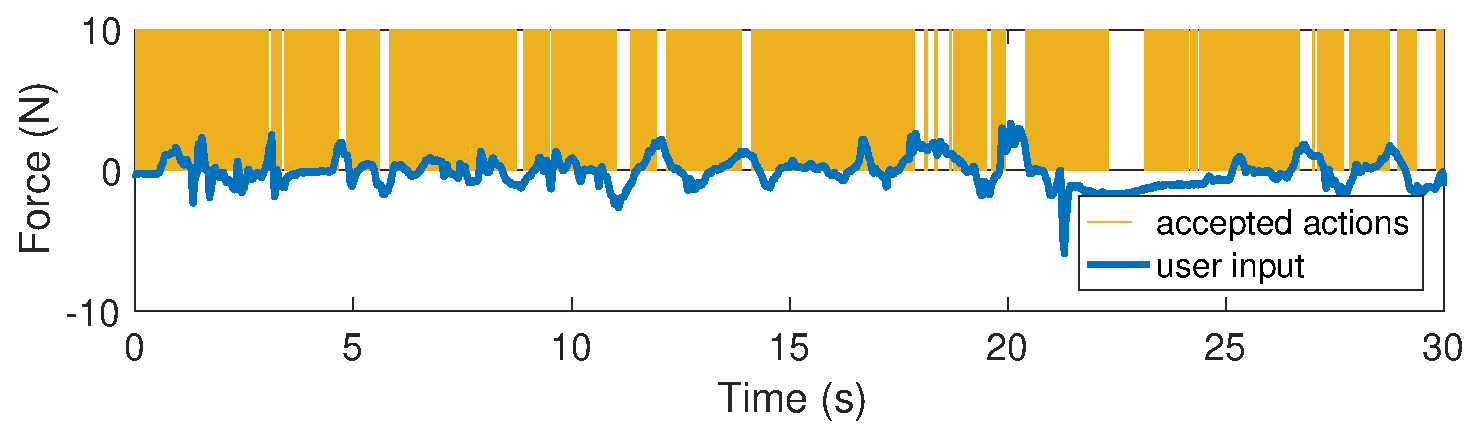
\includegraphics[width=1\columnwidth, keepaspectratio]{ie_good_user_input.eps}
  	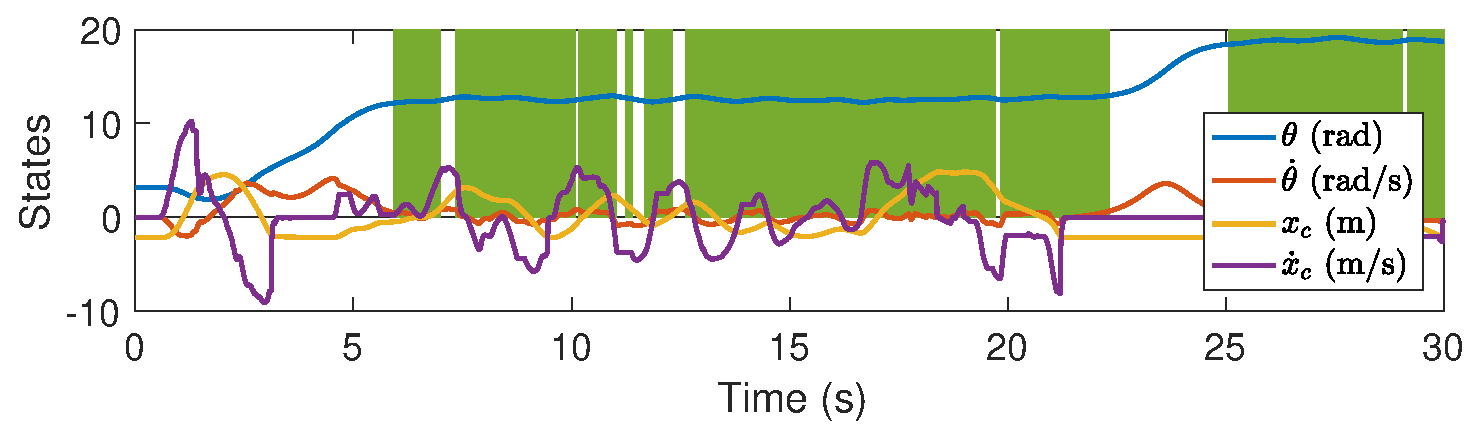
\includegraphics[width=1\columnwidth, keepaspectratio]{ie_good_user_states.eps}
\end{center}
\caption{Example trial data from study. (top) User force input with an indication of allowed actions in yellow. (bottom) System evolution with green highlighting of the time during which success was recorded. Note: Angle wrapping was not used on $\theta$ in the plot above, but it was used in the calculation of all performance measures. }
\label{fig: example_user}
\end{figure}
was recorded as the balance time. Note that when users were successful multiple times in the same trial, time spent in the balance region was cumulative. Lastly, an RMS error of each trajectory generated by the users was calculated with respect to the desired position in an inverted unstable equilibrium (zero-vector of the states). RMS error was normalized by the RMS error of a constant trajectory at the stable equilibrium, equivalent to the error of the user not moving from the initial conditions. 

A percent of rejected actions (PRA) was also recorded. PRA measured the fraction of user inputs that were rejected up to the time of a successful inversion, where we define an action to be a non-zero user input. 

Data from an example trial is visible in Fig.~\ref{fig: example_user}. In this case the trial was successful, with time to success = 8.3s, balance time = 19.7s, and RMS error = 0.57. The PRA was $13\%$.



\chapter{Robotic Assistance with Minimal Interference}
\label{chapter: assistance}

%Whereas during training, we allow users to fail at task completion for improved learning, during assistance in tasks, such as activities of daily living (ADL), we may want to insist on task success, user safety, or both. In these situations, we can modify the proposed filter to actively provide assistance. Instead of using a null controller input as the alternative to user input, we can engage the controller and replace rejected actions with optimal control, calculated by an MPC. In the next two subsections, we provide simulation results that demonstrate system behavior when the MIG-based filter is employed in assistance mode.

When assisting users in physical tasks, there are two highly desired features of a shared control paradigm. For one, we may want to insist on task success, user safety, or both even for unskilled users. Secondly, it should remain as transparent as possible to users at times when they do not require assistance at the task. In the simulation results presented below, we show that the proposed filter-based shared control paradigm in assistance mode possesses both features---it can successfully assist in task completion and/or keep a simulated user safe, while remaining sensitive to the user's skill level and engaging minimally. 

%
%\section{MIG criterion}
%
%Descent proofs. XXX
%
%	\begin{prop}\label{prop:: descent}
%	Consider systems with state $x$ and control $u$ and an objective given by \eqref{eq:: cost_wo_u}. Then, the control policy given by \eqref{eq:: u_alphad} is a descent direction for all $t\in[t_o, t_f]$. Further, if there exists $t\in[t_o, t_f]$ for which the MIG is negative, then the feedback policy in \eqref{eq:: u_alphad} will decrease the cost. Moreover, this feedback policy converges to the local minimizer trajectory, as stated in Definition 1. 
%	\end{prop}
%	\begin{proof}
%	Using a first-order Taylor expansion, we write
%	\begin{equation}\label{eq:: Te1}
%	J_1(v(t) + w(t)) \approx J_1(v(t)) + \frac{\partial J_1}{\partial u(t)}\Big\rvert_{v(t)}\cdot w(t). 
%	\end{equation}
%	For objectives of the form in \eqref{eq:: cost_wo_u}, we use the G\^ateaux derivative to calculate the gradient of the cost with respect to the control 
%	\begin{align}\label{eq:: Te}
%	\frac{d}{d\epsilon}J_1(v(t) + \epsilon w(t))\Big\rvert_{\epsilon=0} =& \int_{t_o}^{t_f} \rho(t)^TB(t)\cdot w(t)\,\mathrm{d}t.\end{align}
%	From \eqref{eq:: Te1} and \eqref{eq:: Te}, the first-order change in cost can be approximated with 
%	\begin{align*}
%	\Delta J_1 \approx \int_{t_o}^{t_f} \rho^T(t) B(t) \cdot w(t) \mathrm{d}t.
%	\end{align*}
%	Equivalently, using \eqref{eq:: MIG_noU}, we can write
%	\begin{align*}
%	\Delta J_1 \approx \int_{t_o}^{t_f} \frac{dJ_1}{d\lambda_+} \mathrm{d}t, 
%	\end{align*}
%	which, with the update of \eqref{eq:: u_alphad} and given that $\alpha_d < 0 $, becomes
%	\begin{align*}
%	\Delta J_1 \approx \int_{t_o}^{t_f} \alpha_d \lVert\rho^T(t) B(t)\rVert_{(\Lambda(t)+R)^{-1}}^2 \mathrm{d}t \le 0.
%	\end{align*}
%
%	We examine the case of the equality, such that 
%	\begin{align*}
%	\Delta J_1 = 0 &\Leftrightarrow \rho^T(t) B(t) = 0~\forall~t\in[t_o, t_f]\\
%	&\Leftrightarrow \frac{dJ_1}{d\lambda_+} = 0~\forall~t\in[t_o, t_f].
%	\end{align*}
%	If there exists $t\in[t_o,t_f]$ for which $dJ_1/d\lambda_+ < 0$, then $\Delta J_1 <0$. 
%	The change in cost, to first order, will be zero if and only if $\rho^T(t) B(t) = 0$ for all $t \in [t_o, t_f]$, which is the condition for a minimum according to Pontryagin's Maximum Principle (for objectives of the form in \eqref{eq:: cost_wo_u}).
%	\end{proof}
%   
%    Next, we prove that one can scale the descent direction in an arbitrary way, differently across the time-horizon, and still obtain a descent direction, provided that the direction of the update is maintained. 
%    
%    \begin{figure}[h]
%	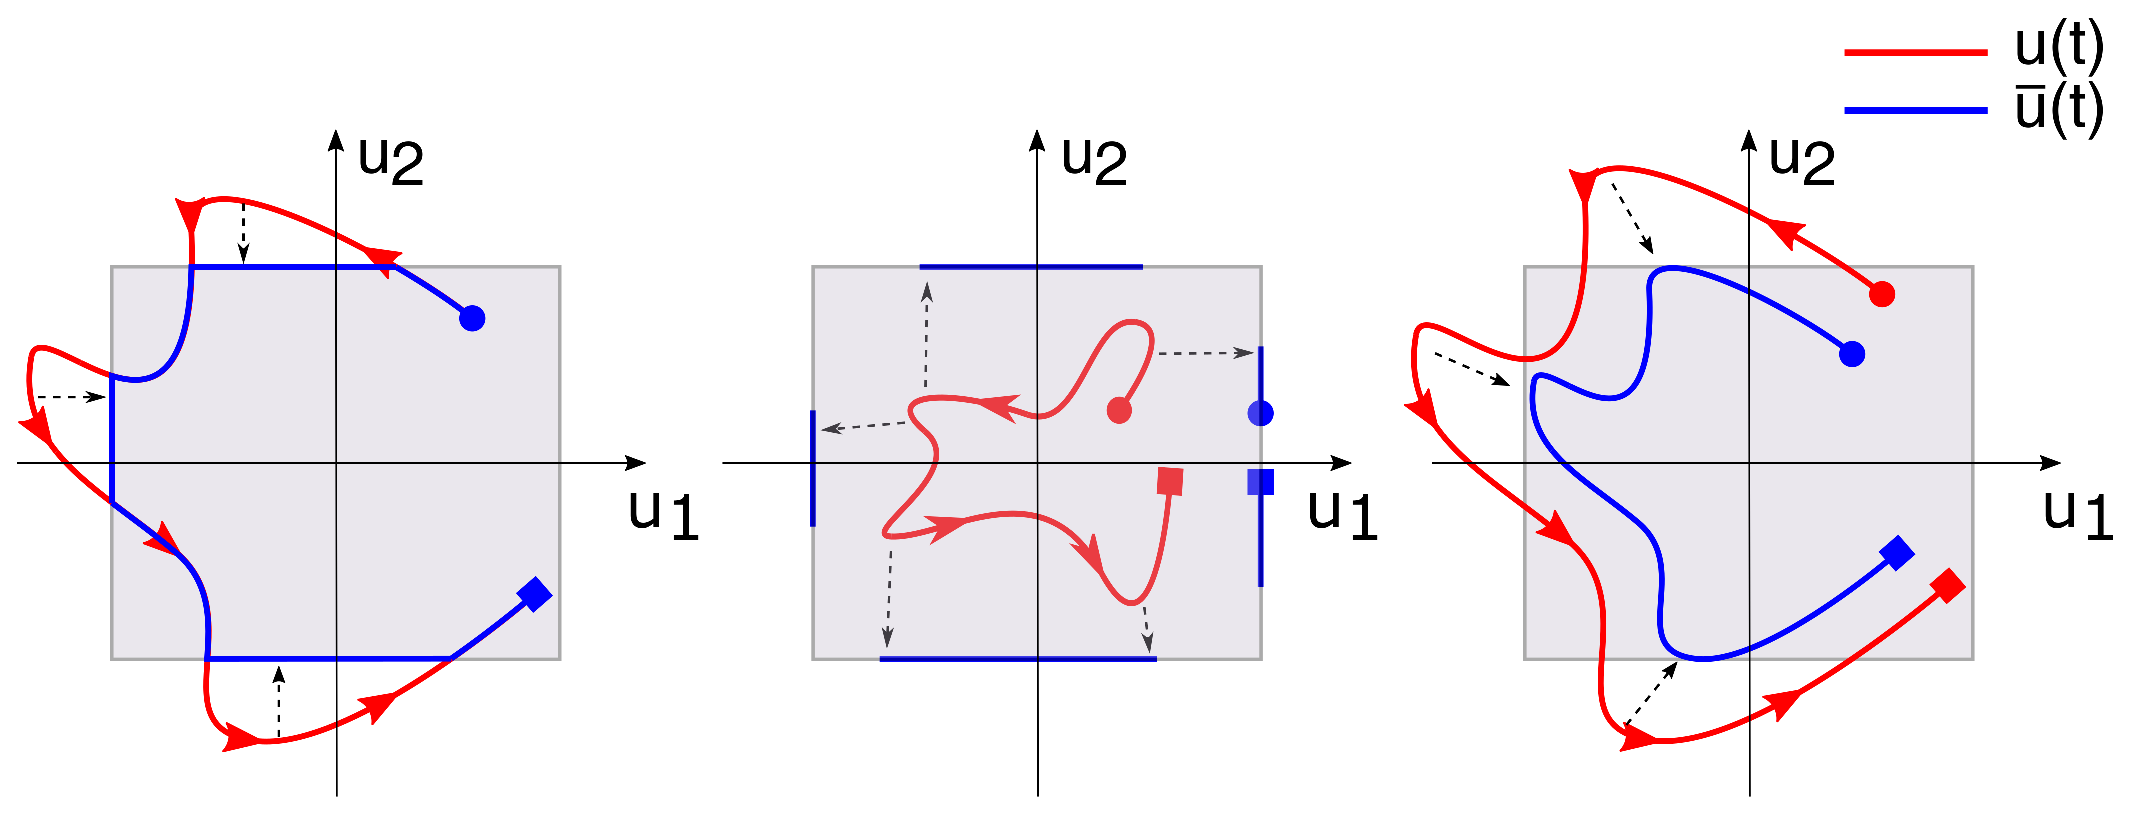
\includegraphics[width=\linewidth, keepaspectratio]{Scaling.eps}
%    \caption{Cases of control scaling that remain valid descent directions for the proposed needle-variation controller. The left figure shows control clipping, where values are saturated at a specific threshold; the middle figure shows arbitrary stretching to the saturation limits; the right figure shows proportional scaling that maintains the same direction of the applied control. Control curves are a function of time and arbitrarily shown for a 2-input system for easier visualization. Simulation results in this paper use control clipping.}
%    \label{fig: Descent Direction}
%    \end{figure}    
%    
%	\begin{prop}\label{prop:: saturated_descent_noad}
%	Consider systems with state $x$ and control $u$ and an objective metric given by \eqref{eq:: cost_wo_u}. Let $\Gamma(t) \succ 0$ be a diagonal matrix. The control update $w(t)$ given by \eqref{eq:: u_alphad} remains a descent direction for the entire trajectory even when scaled to $w_s(t) = \Gamma(t) w(t)$.
%	\end{prop}
%	\begin{proof}
%	Consider the update policy in \eqref{eq:: u_alphad} with scaled control $\bar{u}(t)$. Let $w_s(t)$ indicate the perturbation after scaling, such that $\bar{u}(t) = v(t) + w_s(t)$, where $w_s(t) = \Gamma(t) w(t)$, where the diagonal elements of $\Gamma(t)$, $\gamma_i(t) \ge 0$, can be different from each other.
%	
%	From Proposition \ref{prop:: descent_noad}, the cost change, approximated to first-order, is then
%	\begin{align}\label{eq:: sat_DJ_wa}
%    \Delta J_1 \approx \int_{t_o}^{t_f} \alpha_d \lVert\rho^T(t) B(t)\rVert_{\Gamma(t)(\Lambda(t)+R)^{-1}}^2 \mathrm{d}t.
%    \end{align}
%    Given that $\alpha_d < 0$, $\Gamma(t) \succ 0$, and $\Lambda(t)+R \succ 0$, \eqref{eq:: sat_DJ_wa} is negative if there exists time $t$ in $[t_o, t_f]$ such that $\rho^T(t)B(t)\ne 0~ \iff w_s(t) \ne 0$. Hence, 
%    \begin{gather*}
%    \Delta J_1 < 0 \\\iff \exists~t \in [t_o, t_f]~\text{such that}~w_s(t)=\Gamma(t)w(t)\ne 0. 
%    \end{gather*}
%    Therefore, given the update \eqref{eq:: u_alphad}, the cost---approximated to first-order---is guaranteed to decrease provided that there exists $t \in [t_o, t_f]$ such that $\bar{u}(t) \ne v(t)$.
%    \end{proof}
%    
%    We note that Proposition \ref{prop:: saturated_descent_noad} holds even when control inputs are scaled differently in time. Fig. \ref{fig: Descent Direction} shows valid cases of control distortion that remain a descent direction.
%   



\section{Performance-Oriented Assistance}

Experiments were completed using simulated users attempting the task of cart-pendulum inversion, as described in Section~\ref{section: simulated users} of Chapter~\ref{chapter: methods}. 

\begin{figure}[!t]
\begin{center}
    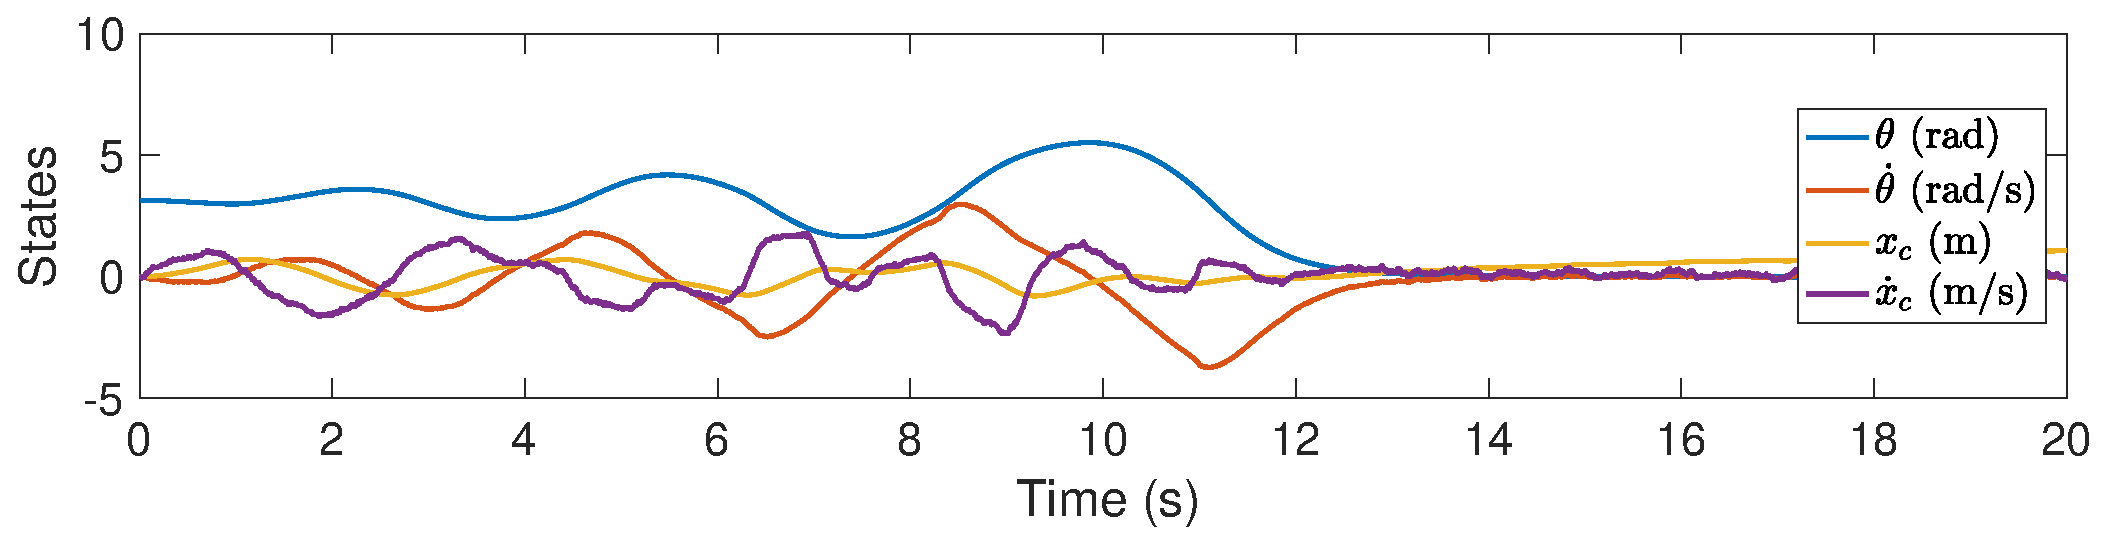
\includegraphics[width=1\columnwidth, keepaspectratio]{MC_states_1.eps}
    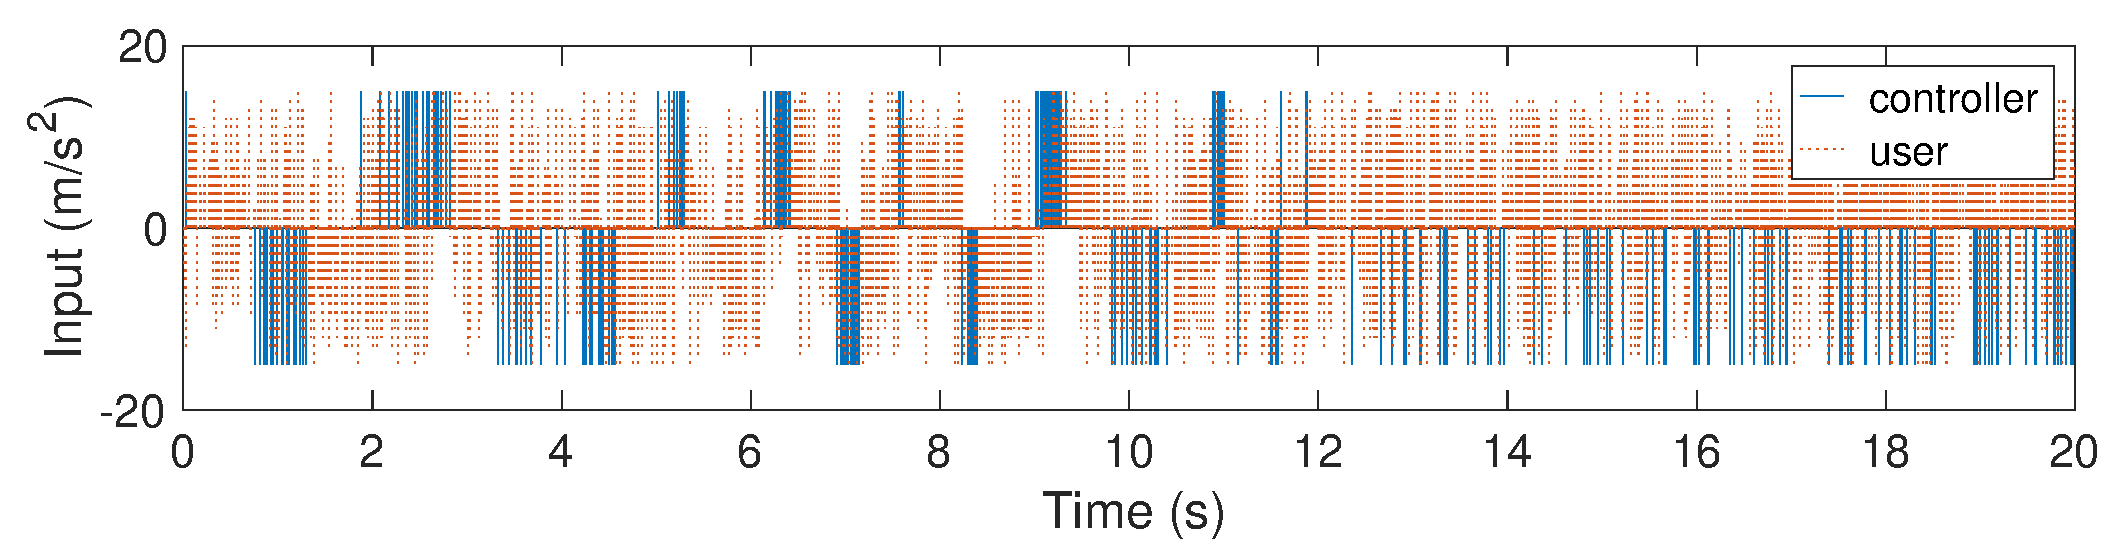
\includegraphics[width=1\columnwidth, keepaspectratio]{MC_control_1.eps}
    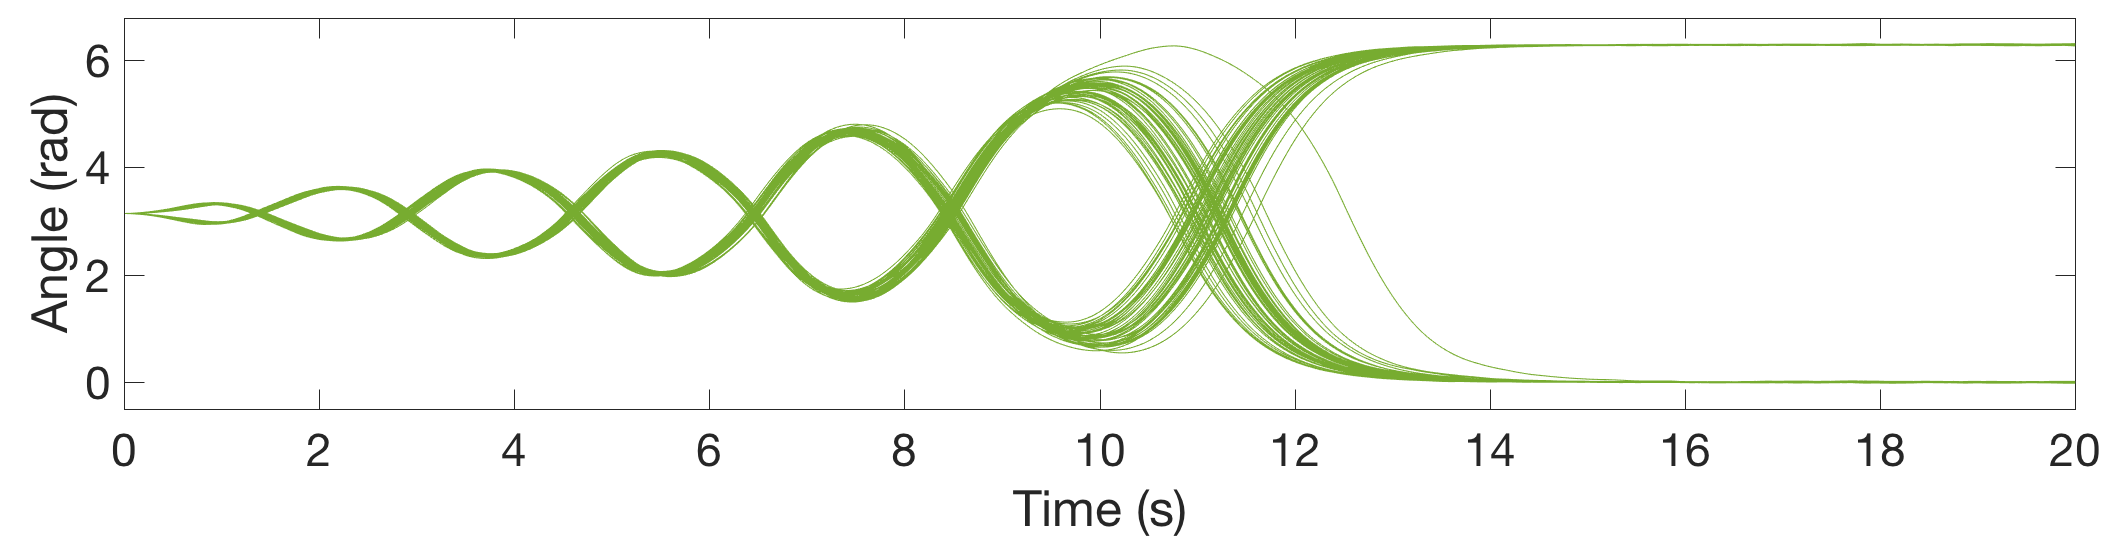
\includegraphics[width=1\columnwidth, keepaspectratio]{MC_angle_100.eps}
\end{center}
\caption{For the cart pendulum inversion task, noise input with a MIG-based filter in assistance mode is able to invert the pendulum in 100 out of 100 of the simulation ran. (top, middle) An example trial with the system evolution and filtered input are shown. (bottom) Convergence results from all 100 trials.}
\label{fig: MC_cp}
\end{figure}

A series of 100 Monte Carlo simulations were run for unskilled users (as modeled using Gaussian noise) attempting the task of cart pendulum inversion. System behavior, simulated user input, and controller intervention during an example trial are visible in Fig.~\ref{fig: MC_cp}. Results of the 100 trials with noise input demonstrate a $100\%$ success rate and are also shown in the figure.

What is more, we are interested in how controller intervention changes according to the skill level of a user. We note close to $0\%$ intervention for a simulated skilled user and $\sim50\%$ intervention for noise input, which makes sense in this one-dimension-controlled task of inverting a pendulum. 

Note that for simulated users the relationship between skill and controller intervention is explicit ($0\%$ intervention for an always successful user and $\sim50\%$ for noise input). With human subjects, such a relationship is more difficult to assess, because we can only approximate users' skill level and cannot account for momentary mistakes. However, we perform an analysis on data collected in a human subject experiment described in Chapter~\ref{chapter: training}. We identify a weak but analogous relationship between subjects' estimated skill level and controller engagement when using the MIG-based filter in training mode. 


\section{Safety-Oriented Assistance}

Next, we analyze the performance of MIG-based assistance on a spring-loaded inverted pendulum (SLIP) model. For our experiments, we use simulated users modeled using MPCs with differing objective functions as described in Section~\ref{section: simulated users} of Chapter~\ref{chapter: methods}. 

We show that with the MIG filter in assistance mode the SLIP can be kept upright even when input is provided by Gaussian noise or a low-skill user. From Fig.~\ref{fig: SLIP_noise} we see that for noise input the filter allows the foot to make random movements and the SLIP to change direction, while keeping the center of mass oscillating around a safe constant height. 


\begin{figure}[!t]
\begin{center}
   	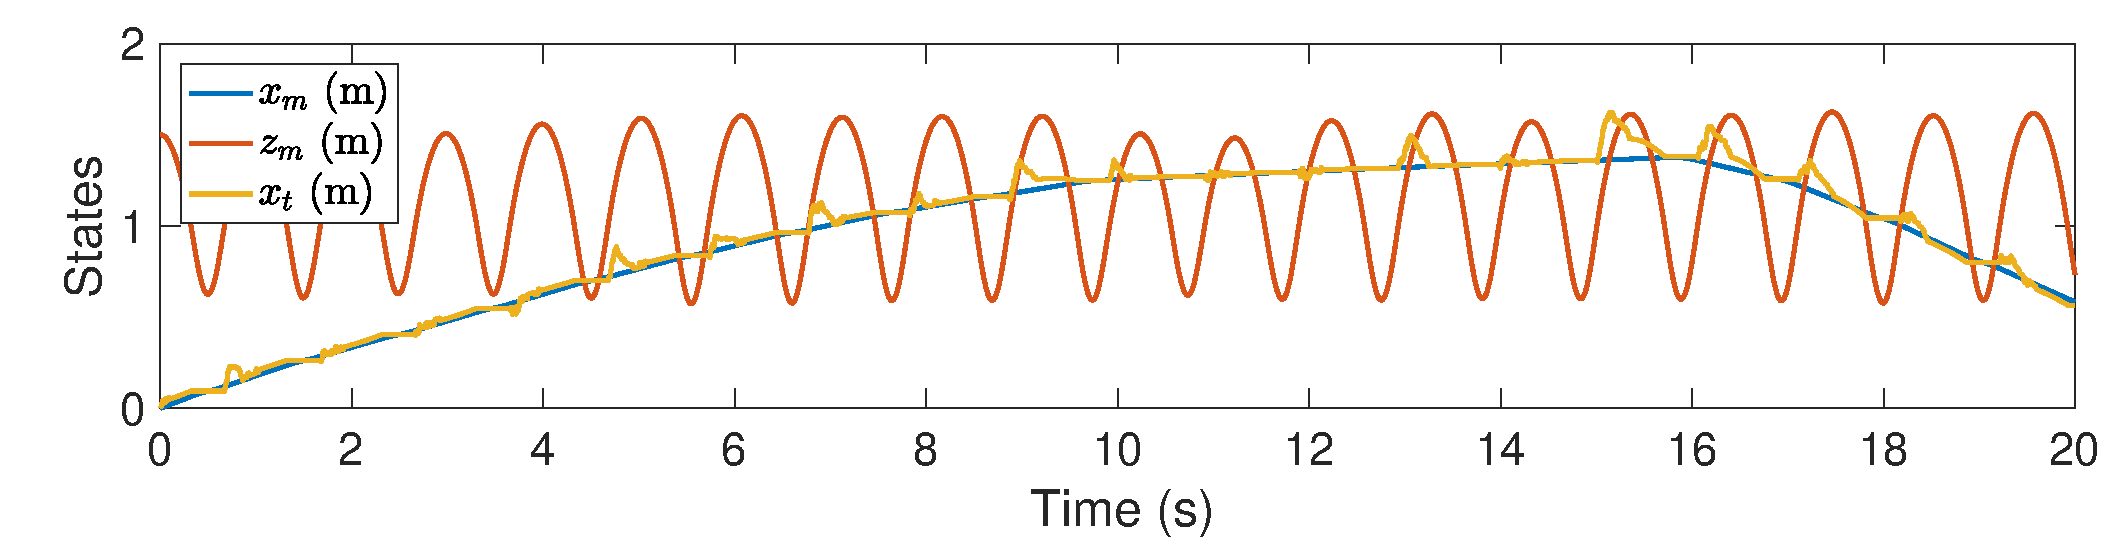
\includegraphics[width=1\columnwidth, keepaspectratio]{SLIP_noise_states.eps}
\end{center}
\caption{We simulate a SLIP model using Gaussian noise as user input and the MIG-filter in assistance mode for support. Note that the filter allows the foot to make random movements and the SLIP to change direction, while keeping the center of mass oscillating around a safe constant height. The controller overrides the user's input for $\sim70\%$ of the simulation time.}

\label{fig: SLIP_noise}
\end{figure}
\begin{figure}[!t]
\begin{center}
  	\includegraphics[width=1\columnwidth, keepaspectratio]{SLIP1_noassist_velocity.eps}
  	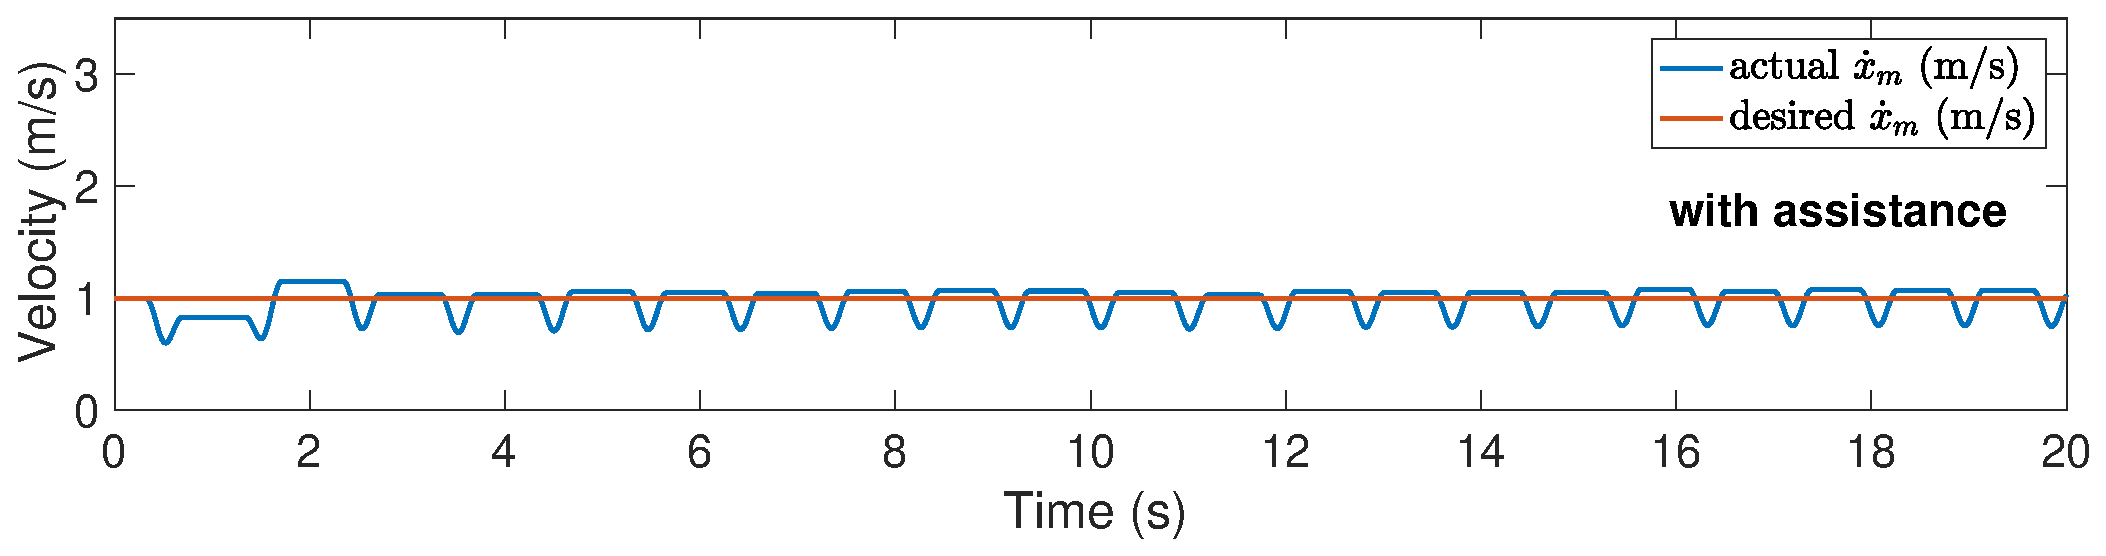
\includegraphics[width=1\columnwidth, keepaspectratio]{SLIP1_assist_velocity.eps}
\end{center}
\caption{(top) We simulate a low-skill user that attempts to move forward with no assistance. The SLIP falls after $\sim5.5s$. (bottom) We use the same user simulation but now the controller helps the user keep balance without restricting its forward motion. With under $40\%$ controller intervention, the SLIP establishes a cyclic gait and maintains an average speed of $0.98~m/s$ (close to the user's desired $1~m/s$).}
\label{fig: SLIP_weak}
\end{figure}

\begin{figure}[!t]
\begin{center}
   	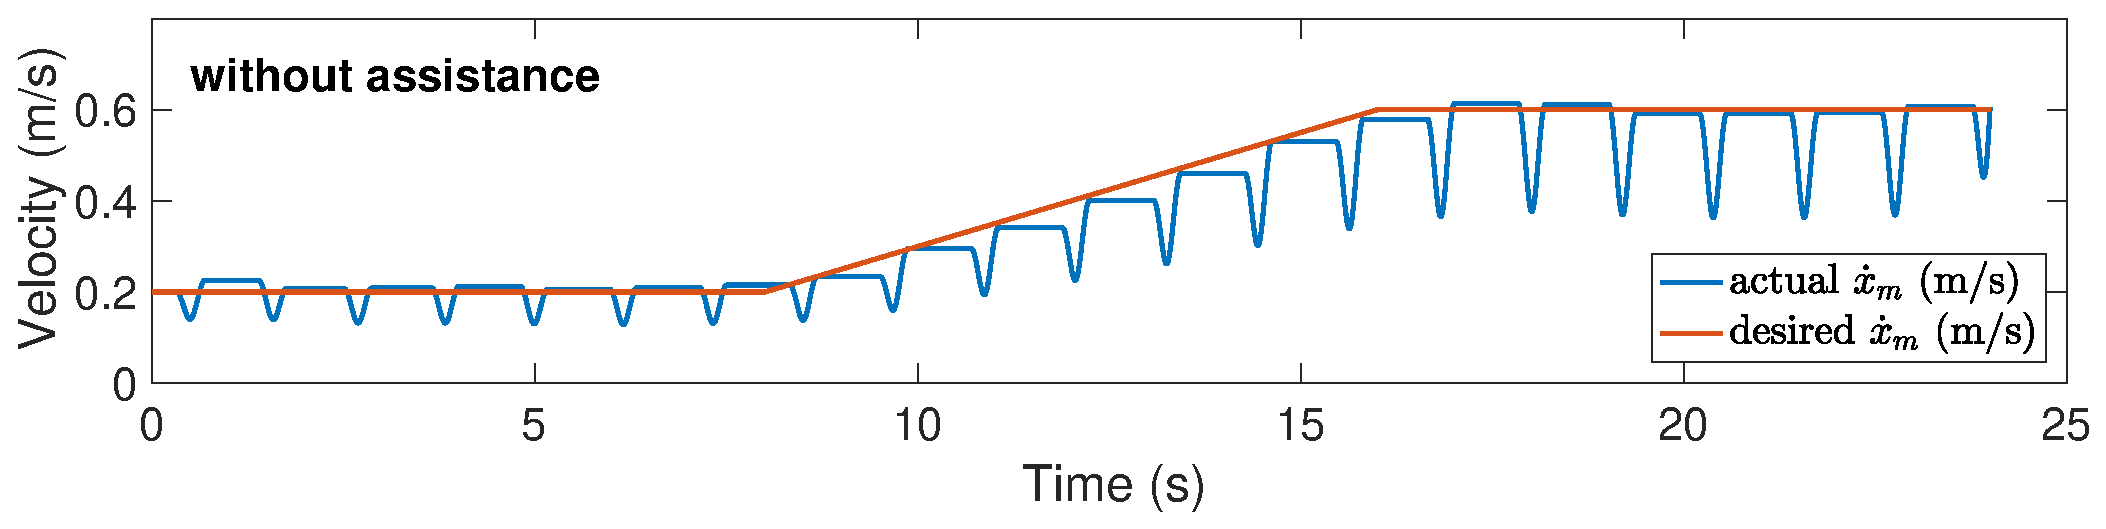
\includegraphics[width=1\columnwidth, keepaspectratio]{SLIP2_noassist_velocity.eps}
   	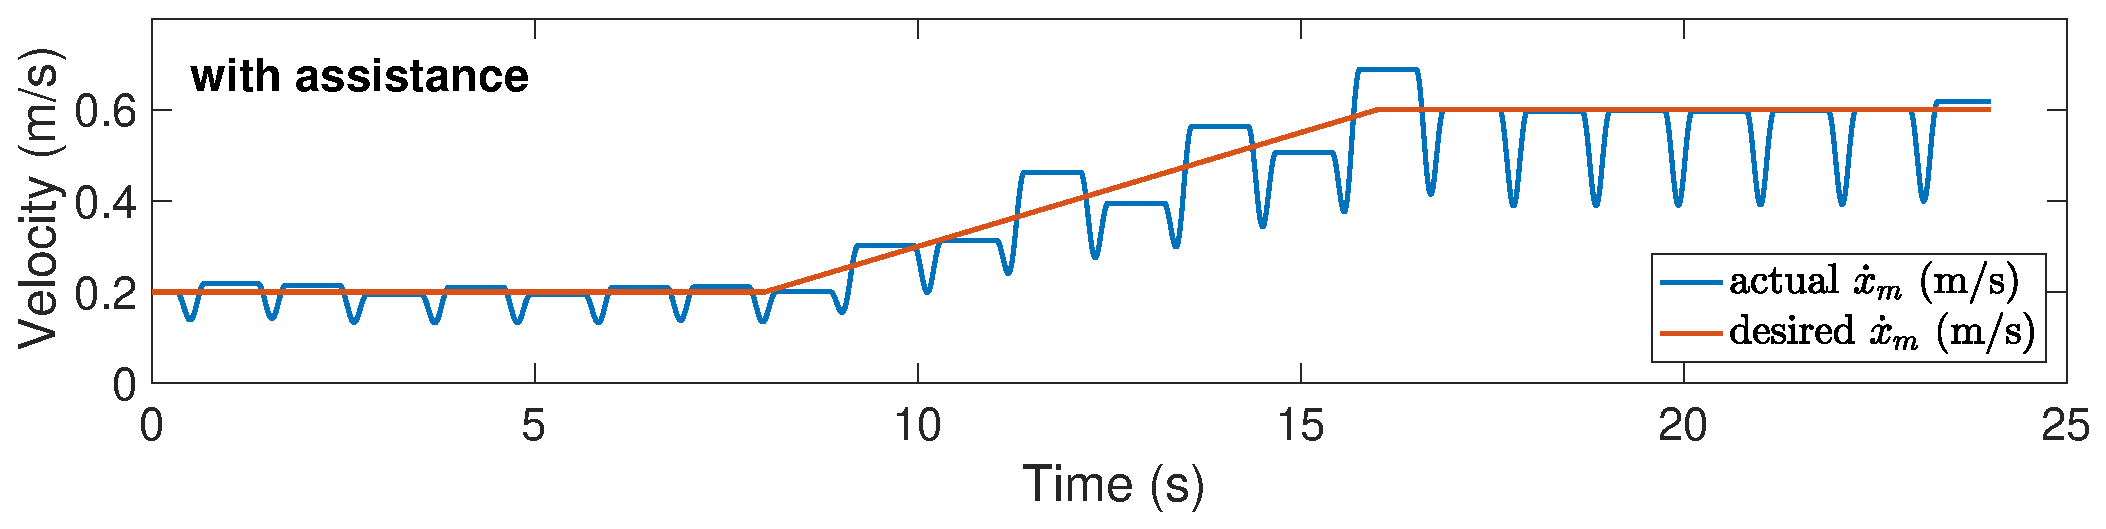
\includegraphics[width=1\columnwidth, keepaspectratio]{SLIP2_assist_velocity.eps}
\end{center}
\caption{(top) We simulate a capable user that attempts to move forward with varying velocity. (bottom) We simulate the same user with added assistance. Note that the assistance does not impede the user's forward motion, even though the controller has no \textit{a priori} knowledge of the user's desired velocity. The controller intervenes $\sim~20\%$ of the time.}
\label{fig: SLIP_skilled}
\end{figure}

For a low-skill user, the assistance prevents the SLIP from falling, while allowing it to maintain its desired forward velocity, as visible in Fig.~\ref{fig: SLIP_weak}. Finally, when provided with input from a skilled user, the filter allows the user to dictate its desired forward velocity and interferes only minimally with its desired motion, as visible in Fig.~\ref{fig: SLIP_skilled}. 

What is worth noting is that the controller overrides user input for $\sim70\%$ of the time for noise input, for under $40\%$ of the time for a low-skill user, and for $\sim~20\%$ of the time for a skilled user. Again, we see a relationship between the skill of the user and controller engagement. The more skilled a user is at the task, the less the controller interferes, while even for noise input the controller is able to keep the hopper upright and safe. 

Based on these results, the MIG criterion shows promise to be used in assistance-oriented applications, such as lower-limb exoskeletons \cite{exoskeletons}. In walking assistance, we want to at all cost prevent users from falling, while at the same time giving them freedom to follow their natural gait pattern, walk at a desired pace, and change speeds or stop when convenient. Such an implementation of the shared control paradigm will be evaluated in future work. 



\chapter{Training Through Forceful Interaction}
\label{chapter: training}

%Whereas during training, we allow users to fail at task completion for improved learning, during assistance in tasks, such as activities of daily living (ADL), we may want to insist on task success, user safety, or both. In these situations, we can modify the proposed filter to actively provide assistance. Instead of using a null controller input as the alternative to user input, we can engage the controller and replace rejected actions with optimal control, calculated by an MPC. In the next two subsections, we provide simulation results that demonstrate system behavior when the MIG-based filter is employed in assistance mode.

Whereas during assistance, we prevent users from failing at a task, during training we may want to allow failure for improved learning. In these situations, we can use the proposed filter without actively providing assistance. Instead of using a calculated controller input as the alternative to user input, we can simply reject ``wrong" user actions and wait for the user to figure out the ``correct" next action. 

In the following chapter, we demonstrate results of a human subject study, where we compare learning of the cart-pendulum inversion task between a group training with feedback in the from of the filter-based shared control and a group training for an equivalent duration of time without feedback. Details of how the experiment was set up can be found in Section~\ref{section: human experiments} of Chapter~\ref{chapter: methods}.

\section{Training Effect}

\begin{figure}[!h]
	\begin{center}
		\includegraphics[width=\columnwidth]{training.pdf}
	\end{center}
	\caption{There was a training effect from training with the filter-based feedback compared to training with no feedback. The RMS error, balance time, and time to success of the training group in the final set was significantly better than that of the control group. It is also worth noting that as expected, pairwise comparisons of the two groups in set 1 show that there was not a significant difference in their baseline performance measurements. Moreover, set was consistently the most significant factor in performance improvements from set 1 to set 3, showing that both groups (training and control) improved significantly over time. Finally note that error bars indicate standard error and significance is indicated by $^*p<0.05$, $^{**}p<0.01$, $^{***}p<0.001$.}
	\label{fig: training}
\end{figure}

The main result we were looking for in the study was whether providing filter-based feedback through forceful interaction would improve learning. And indeed, we observed a significant training effect from training with filter-based feedback compared to training with no feedback for an equivalent duration of time, as visible in Fig.~\ref{fig: training}. \textit{Post hoc} analysis confirmed that both groups started the experiment at comparable skill levels and although training time was the main factor impacting improvement in performance (both groups improved over time), the training group improved significantly more than the control. Detailed statistical analysis is described below. 

A two-factor repeated measures ANOVA was used to assess the effects of the group (between-subjects) and set (within-subjects) on all performance measures listed in Section~\ref{metrics} of Chapter~\ref{chapter: methods}. The training group and control group were evaluated based on set 1 and set 3 only. Set 2 was left out of the ANOVA, so that effects of the assistance itself would not be measured in the analysis. Additionaly, pairwise comparisons were made between set 1 for both groups, between set 3 for both groups, and between set 1 and set 3 within each group using a paired 2 sample t-test. 

Firstly, we confirmed that there was on average no difference in skill at the onset of the experiment. Pairwise comparisons within each of the four measures (success rate, RMS error, balance time, and time to success) showed that in set 1 there was not a significant difference between the training group and control group. For instance, the main effect of group in set 1 on the RMS error was not significant ($F(1,26)=1.615, p = 0.215$)---there was not a significant difference between the training group ($mean =0.612, SD =0.088$) and the control group ($mean = 0.639 , SD=0.067$) in set 1. The same was true for the three other metrics. According to 2-sample t-tests, the differences between the two groups were also not significant across all 4 metrics ($p>0.01$).

Secondly, we found that time had the most significant impact on learning. The factorial ANOVA revealed that for success rate the main effect of set yielded an F ratio of $F(1,50)=7.555,\ p=0.008$, meaning that users were more successful in set 3 ($mean =0.280 , SD = 0.223$) than in set 1 ($mean = 0.140,\ SD = 0.100$) regardless of the type of practice in set 2. Similarily, the RMS error showed that the main effect of set yielded an F ratio of $F(1,26) = 41.551, p<0.001$, indicating a significant difference between set 1 ($mean =0.651, SD =0.085$) and set 3 ($mean =0.599, SD =0.072$). The main effect for set on the balance time yielded an F ratio of $F(1,26)=15.328,\ p<0.001$, indicating a significant difference between the balance time in set 1 ($mean = 0.408, SD = 1.053$) and set 3 ($mean = 0.866, SD = 1.476$). The main effect of set on time to success was also significant ($F(1,26)=18.992,\ p<0.001$), with set 3 ($mean = 27.830, SD = 4.433$) outperforming set 1 ($mean = 28.955,SD =3.175$). Set had a significant effect on increases across all metrics, indicating that participants were continuously improving with time regardless of the feedback that was provided. 

Thirdly, we observed that there was more improvement among members of the training group than control. When training group and control group were compared in set 3 using 2-sample t-tests, the training group performed better. The set 3 balance time of the control group ($mean =0.632, SD = 1.261$) was significantly less ($t(728)=3.643,p<0.001$) than the balance time of the training group ($mean = 0.994 , SD = 1.568$). The time to success was also significantly better ($t(738)=3.110, p=0.002$) in set 3 of the training group ($mean = 27.500, SD = 4.744$) compared to set 3 of the control group ($mean =28.43, SD = 3.74$). The same was true for the RMS error ($t(699)=-8.919,p<0.001$)---the RMS error of the training group in set 3 ($mean = 0.58, SD = 0.003$) was lower than the RMS error of the control ($mean = 0.63, SD = 0.004$). The RMS error, balance time, and time to success of the training group in the final set was significantly better than that of the control, while the difference for success rate was not statistically significant. 

Moreover, the RMS error showed that there was a significant interaction effect between group and set ($F(1,26)=5.099, p=0.0326$). This is indicated in Fig.~\ref{fig: training} by the two groups having similar means in set 1 but significantly different means in set 3, implying that the training had a greater impact on set 3 performance than the unassisted practice of the control group. For the other measures, the interaction effects were statistically insignificant---there was no significant interaction effect of group and set on balance time ($F(1,26)=1.048,\ p=0.315$), time to success ($F(1,26)=1.512,\ p=0.22983$) or success rate ($F(1,50)=0.111,\ p=0.740$). There was also no signifcant effect of group on any of the metrics: success rate ($F(1,50)=0.981,\ p=0.327$), balance time ($F(1,26)=1.562,\ p=0.223$), time to success ($F(1,26) = 1.114,\ p=0.301$), or RMS error ($F(1,26) = 1.824 ,\ p=0.189$). In summary, although there was not a significant effect of group on any of the  metrics, the RMS  error  showed  that there  was  a  significant  interaction  effect between  group  and set.  

% Although the change in success rate from set 1 to set 3 was significant for both the control group ($t(9)=3.152,\ p = 0.012$) and the experimental group ($t(17)=3.127,\ p=0.006$), the effect size of the training group ($d=0.94$) from set 1 to set 3 was larger than the effect size of the control group ($d=0.77$). (XXX why report this only for success rate?) 

 % Note that the control group continued to improve their success rate with each set, possibly because their interaction with the robot did not change between sets as it did for the training group. 


\begin{figure}[!h]
	\begin{center} 
	\begin{multicols}{2}
		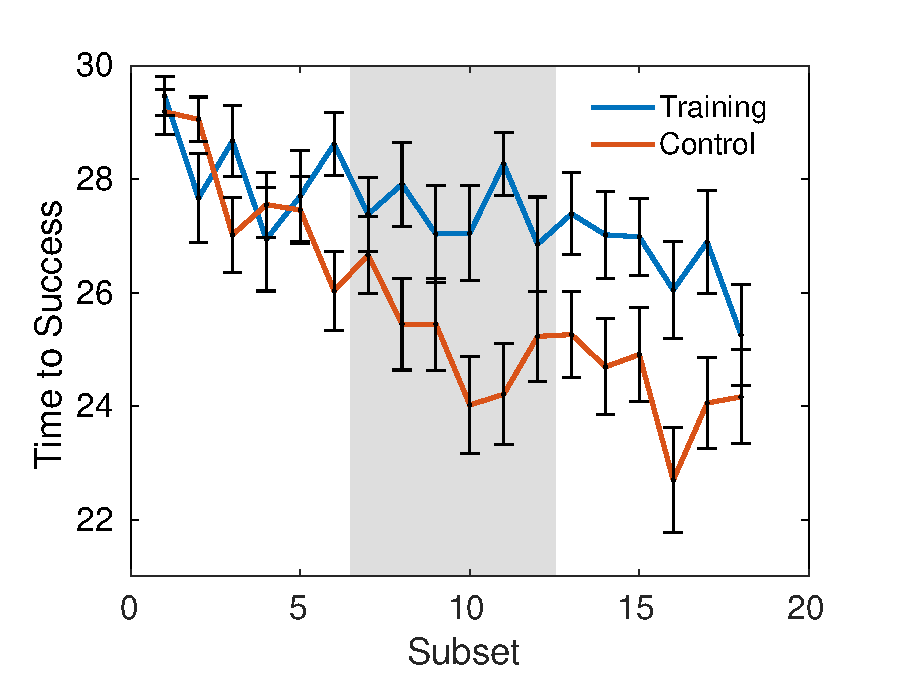
\includegraphics[width=0.85\columnwidth]{tts_plateau.eps}
		\caption*{}
		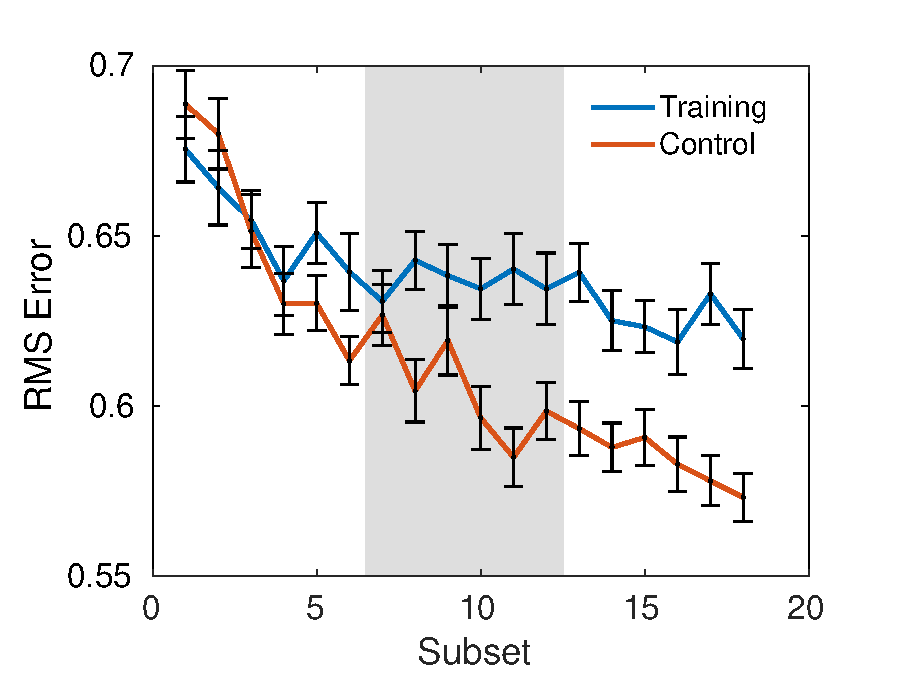
\includegraphics[width=0.9\columnwidth]{err_plateau.eps}
		\caption*{}
	\end{multicols}
	\end{center}
	\vspace{-1.2cm}
	\caption{Grey band covers subsets included in set 2 (the set, where the training group received feedback). Note that training and control groups showed similar improvement during set 1, while the training group showed faster improvement during set 2. Particularly with respect to the RMS error, the control group's improvement slows down drastically during set 2, while the training group keeps improving.}
	\label{fig: plateau}
\end{figure}


Finally, in order to assess how subject performance evolved over time, the baseline and post-training sets were analyzed using subsets containing five individual trials, rather than the sets of thirty trials used for the analysis above. As such, there were 6 subsets in each set as shown in Fig.~\ref{fig: plateau}. We can see that the training and control groups diverage in performance during the subsets of set 2. Particularly with respect to the RMS error, the control group plateaus in improvement while the training group keeps improving. These results support the hypothesis that subjects experience accelerated learning while receiving feedback through filter-based forceful interaction. 

 
\section{Real-Time Performance Improvement}

Like detailed in the section above, the two experimental groups performed similarly in their baseline trials. However, in set 2, the group using the filter outperformed the control group in terms of time to success, RMS error, and balance time.

The experimental group ($mean = 25.168, SD = 7.686$) had a lower time to success ($t(798.03) = -4.999, p = 7.067 \times {10}^{-7} $) than the control group ($mean = 27.418, SD = 5.266$). The RMS error of the experimental group ($mean = 0.605, SD = 0.087$) was also significantly lower ($t(753.59) = -5.925, p = 4.738 \times {10}^{-9} $) than that of the control group ($mean = 0.636, SD = 0.066$). Finally, the balance time of the experimental group ($mean = 2.358, SD = 3.469$) was higher ($t(691.51) = 7.28, p = 9.1 \times {10}^{-13}$) than that of the control group ($mean = 1.026, SD = 1.418$), showing that the filter was able to effectively assist subjects in the task and improve all task-specific metrics. There was no significant difference between the success rate of the control group and the experimental group during set 2 ($p = 0.335$), which makes sense because success rate can only be calculated per set rather than per trial and hence many less samples are available. Comparisons between the control and experimental groups are shown in Fig.~\ref{fig: training}. Overall, these results demonstrate that the MIG filter meets the commonly reported requirement of shared control schemes in that it assists subjects with the task while in use. 
 
 
\section{Features of Assist-As-Needed}
\label{skill correlation}

Like described in the Introduction in Chapter~\ref{chapter: intro}, studies emphasize the need for training interfaces to be assist-as-needed. This real-time adjustment to user performance is critical due to two factors:
\begin{enumerate}
\item users start at different skill levels requiring different levels of feedback and assistance
\item users exhibit varying performance levels over time because of either overall improvement at the task or temporary distractions and fatigue again requiring adequately adjusting levels of shared control.
\end{enumerate}
By remaining sensitive to user skill and current performance, the interface avoids overreliance on the assistance and encourages learning. Uniquely in comparsion to most available solutions, it adjusts its engagement on an instantenous basis without the need to specify or approximate additional parameters, such as machine trust in the user. In the sections below, we report experimental results that demononstrate correlations between controller engagement and both initial skill level and within-trial performance.


\subsection{Correlation with Initial Skill Level}

From the experimental results, a relationship was observed between participant skill level---estimated based on performance in unassisted trials---and the frequency of controller intervention in the training set. In this case, we calculate the success rate of the 30 trials from set 1 to approximate user skill level. We then use percent of rejected actions (PRA) values from individual trials in set 2 from the same users to identify the correlation---a scatter plot with the results is visible in Fig.~\ref{fig: MDA_corr_dotproduct}. A Pearson product-moment correlation coefficient was computed and a low negative correlation ($r=-0.14$, confidence interval $(-0.22)-(-0.06)$, $p=0.001$) was identified between overall success rate in set 1 and PRA in individual trials of set 2 for the training group ($n=18$). Similar but weaker correlations were identified between controller intervention and other task-specific metrics, such as balance time ($r=-0.09$, confidence interval $(-0.17)-(-0.007 )$, $p=0.03$) and time to success ($r=0.11$, confidence interval $0.086-0.25$, $p=0.01$).

Since subjects showed significant improvement during set 1 while getting used to the task and testing platform, we ran the same statistics using only the last 10 trials of set 1 to estimate participant skill level. Again, a Pearson product-moment correlation coefficient was computed and a low negative correlation ($r=-0.23$, confidence interval $(-0.31)-(-0.14)$, $p=1.0\times 10^{-7}$) was identified between overall success rate in the last 10 trails of set 1 and PRA in individual trials of set 2. Similar correlations were identified between controller intervention and other task-specific metrics, such as balance time ($r=-0.14$, confidence interval $(-0.23)-(-0.06)$, $p=0.0007$) and time to success ($r=0.24$, confidence interval $0.16-0.32$, $p=1.2\times 10^{-8}$).


\begin{table}[!h]
\begin{tabular}{c|c|c|c}
\textbf{Measure} & Test Sign & $\mathbf{r}$ & $p$ \\
\hline \hline
Success Rate & $-$& $\mathbf{-0.23}$ &  $1.0\times 10^{-7}$ \\
Balance Time & $-$& $\mathbf{-0.14}$ & $0.0007$ \\
Time to Success & $+$ & $\mathbf{+0.24}$ & $1.2\times 10^{-8}$ \\
%Error & $+$ & $\mathbf{-0.007}$ & $0.86$ \\
\end{tabular}
\vspace{0.7cm}
\caption{Correlation results between initial skill level and controller engagement. Pearson's correlation tests were performed by applying a linear model to the participant skill level, as estimated from performance measures in the last 10 trials of set 1, and the frequency of controller intervention in the training set---the PRA in set 2. The expected sign of the correlation coefficient ($r$) for a shared control scheme that is sensitive to the performance of the user is indicated in the column on the left. There was a weak but significant correlation between the current performance of the user and PRA for success rate, balance time, and time to success. For RMS error, results were statistically insignificant ($p=0.86$). }
\label{tab: initial skill}
\end{table}

\begin{figure}[!h]
	\begin{center}
		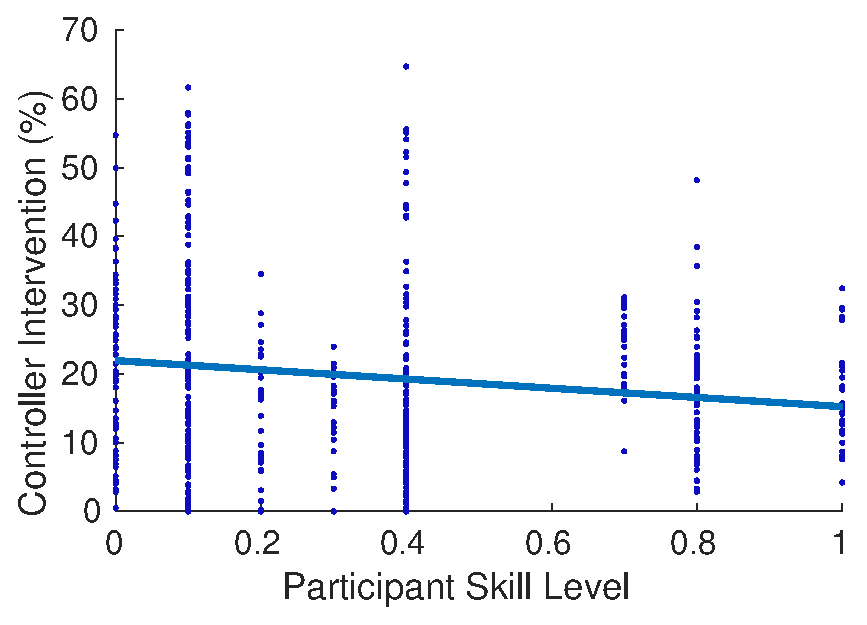
\includegraphics[width=0.8\columnwidth, keepaspectratio]{corr_plot_SKILLvsPAA.eps}\par
	\end{center}
	\caption{A correlation coefficient of $-0.23$ is observed between the success rate of the users in set 1 with no assistance and the rejection rate of the users' inputs in set 2 with assistance, suggesting a correlation between the users' adeptness at the task and the controller's intervention rate during assistance. }
	\label{fig: MDA_corr_dotproduct}
\end{figure}

Overall, for an experimental group of 18 participants, we obtained low but significant correlations \cite{cohen_statistics} between independently measured performance metrics and rejection rate (PRA) in assisted trials, suggesting a relationship between the users' skill level and the MIG filter's rate of intervention. Because the correlations are weak, additional subjects and analysis of other tasks are needed before the skill sensitivity is conclusive. However, our initial findings suggest that a MIG-based filter is a skill-sensitive paradigm that can be used for shared control. MIG-based feedback resembles assist-as-needed shared control schemes, which have been in previous studies shown to be advantageous for learning. 


\subsection{Correlation with User Performance}

Since the filter adjusts on an instaneous basis, we also looked at how it would adapt to a user's overall performance during engagement. We found a weak correlation ($r=0.17$) between the success rate and percent of rejected actions, which demonstrate that the controller engages less often when the user is performing better at the task. Correlation coefficients for other metrics were statistically insignificant, so more testing would have to be conducted to further evaluate the filter. 

Overall though, these results suggest that the proposed filter exhibits features of assist-as-needed paradigms both in terms of adaptation to initial user skill level and adaptation to real-time performance. 



\chapter{Conclusions and Future Work}
\label{chapter: conclusions}

A variety of shared control paradigms have been implemented to provide feedback and assistance to users in settings where the task is known \textit{a priori}. Although users might prefer to maintain control and user engagement is necessary for learning, many applications require a certain level of control authority to be allocated to the machine in order to guarantee safety, improve successful task completion, and/or accelerate learning. As such, most interfaces employ support strategies that in various ways restrict or adjust users' actions in order to enable the subject and the device to move in a safe and constructive manner. 

In this work, we present and evaluate an assessment criterion for user input that can be used in these shared control paradigms. We carry out experiments by using the MIG as an evaluation criterion in a filter-based shared control scheme, similar to \cite{hapticsharedcontrol_review, MDA_Katie}, where user actions deemed by the filter as incorrect are either blocked or hindered by the hardware interface. With only current state information, our proposed filter can both reject unhelpful inputs and remain transparent to operators with significant skill avoiding unnecessary interference improving safety or accelerating training. 

An important feature of the presented interface is its adaptability in real-time. It requires no predefined trajectory, runs on an indefinite time horizon, and automatically adapts to operator skill. It can, like existing adaptive methods, enhance performance while avoiding some of the common long-term pitfalls of ``static" automation such as over-reliance, skill degradation, and reduced situation awareness \cite{adaptive_review}. For complex tasks that require human operators, such as operating a crane or flying an aircraft, these features can alleviate or minimize the need for training with virtual simulators by ensuring safety of the physical system in action. For therapeutic applications, a MIG MDA interface may accelerate recovery or provide assistance by preventing patient slacking, relieving frustration, and utilizing intentioned but noisy signals (e.g., tremor and spasticity) of patients with sensorimotor disorders. Particularly during support in dynamic tasks, such as walking with an exoskeleton, the algorithm can help provide meaningful assistance and ensure safety of the operator-machine system without limiting the user's freedom to maneouver while coupled with the device. 

In future work, the proposed evaluation criterion and filter-based shared control scheme should be explored further. Experimental and theoretical work with MDA in assistance mode should be conducted to establish whether guarantees can be made about the safety of the human-machine system. Further experiments should be carried out to make direct comparisons of MIG MDA to other assist-as-needed controllers. Additionally, we would like to explore other objective functions, such as ergodic objectives or barrier functions, instead of currently used quadratic cost on state to test whether we can make the interface even less restrictive to the users' chosen strategies. At the same time, subjects should be tested in higher dimensional tasks to see if all features of the paradigm hold true even when task complexity increases. And lastly, studies of impaired subjects training in clinically relevant tasks should be performed. 



% Uncomment the 'singlespace' environment and '\bibsep' command
% if needed - some bibliographic styles overide the definition
% of 'thebibliography' in nuthesis.cls
%
%\begin{singlespace}
%\bibsep 12pt
\clearpage\phantomsection % needed for hyperlikns to work correctly

%\begin{thebibliography}{xxx}
%
%\bibitem{label1} A bibliographic item.  A bibliographic item.  A
%bibliographic item.  A bibliographic item.
%\bibitem{label2} Another bibliographic item.  
%\bibitem{label3} Yet another bibliographic item.  
%% The usages of \bibitem and \cite{..} are 
%% explained in Section 4.3 (page 73) of % LaTeX manual.
%% Or you may use BibTeX.
%\end{thebibliography}
%\end{singlespace}

% (The following suggested by Francisco Iacobelli - 5/11/2010)
% In case, you want to use BibTeX, you should replace (or comment)
% the bibliography environment.
% Instead uncomment the following 3 lines and replace <bib file>
% with your .bib file:
\renewcommand\refname{\begin{centering}References\end{centering}}
\bibliography{references}

\bibliographystyle{plain}%IEEEtran}
%\bibliography{IEEEabrv,nxr}

%
%\appendix		% Appendix begins here (optional).


\end{document}
